
\section{MacDonald's solution: transcritical flow with a shock}

This is a MacDonald's steady flow test involving a shock in a short channel. This test was used by Delestre et al.~\cite{Delestre-etal2012} in their \textsc{SWASHES} benchmark library of shallow water analytical solutions. The original derivation of the analytical solution was given by MacDonald et al.~\cite{MBNS1995, MBNS1997}.
MacDonald's analytical solution was derived using a backward framework, that is: given the water depth, we construct the topography which satisfies the shallow water equations.

When water is in a steady state, we have a fixed depth and velocity with respect to time. Consider a one dimensional domain. Suppose that we are given the depth $h(x)$. The steady state conditions make the shallow water equations to the single identity
\begin{equation}
z_x = \left(  \frac{q^2}{gh^3} -1 \right) h_x - S_f
\end{equation}
where $q=uh$ is the momentum or water discharge and $S_f$ is the symbol for the force of bottom friction involving Manning's coefficient $n$. We take 
\begin{equation}
S_f = n^2 \frac{q|q|}{h^{10/3}}.
\end{equation}
The topography is then determined by
\begin{equation}
z(x) = -\int_{x}^{L} z_x~dx
\end{equation}
in which $L$ is the channel length.

\subsection{Results}

For our test, suppose that the channel length $L = 100$ and at steady state the discharge $q = 2$. The initial condition is $u=v=0$ and $w=2.87870797$. The boundary condition is enforced such that the upstream boundary has $q=2$ and the downstream boundary has $h=3.58431872$. When water is steady, suppose that a shock occurs at $x=66\frac23$. Following Delestre et al.~\cite{Delestre-etal2012}, we consider the water depth
\begin{equation}
h(x,y)= \left\{ \begin{array}{ll}
       \left( \frac{4}{g}\right)^{1/3} 
       \left(\frac43 - \frac{x}{100}  \right) - \frac{9x}{1000} \left( \frac{x}{100} -\frac23 \right)
        & ~\textrm{if}\quad 0 \leq x < 66\frac23\\
        ~~ & ~~ \\
       \left( \frac{4}{g}\right)^{1/3}
       \left[ a_1\left( \frac{x}{100} -\frac23 \right)^4 +a_1\left(  \frac{x}{100} -\frac23 \right)^3 \right.\\
       \left. \quad -a_2 \left( \frac{x}{100} -\frac23 \right)^2 + a_3 \left( \frac{x}{100} -\frac23 \right) +a_4\right] 
       & ~\textrm{if}\quad 66\frac23 \leq x \leq 100\\
\end{array} \right.
\end{equation} 
where 
$a_1 = 0.674202$, 
$a_2 = 21.7112$, 
$a_3 = 14.492$, 
$a_4 = 1.4305$, and 
$n  = 0.0328$.


The following three figures show the stage, $x$-momentum, and $x$-velocity when water is steady. We should see excellent agreement between the analytical and numerical solutions.

\begin{figure}
\begin{center}
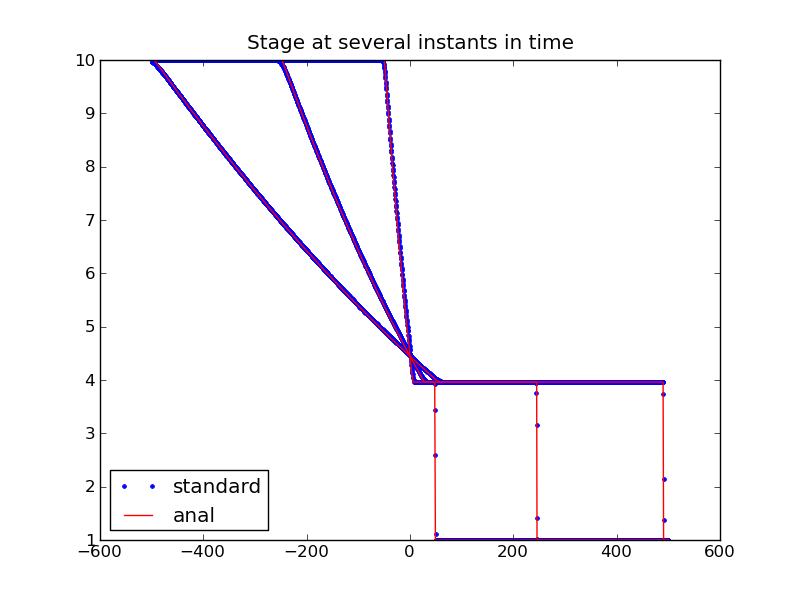
\includegraphics[width=0.9\textwidth]{stage_plot.png}
\end{center}
\caption{Stage results}
\end{figure}


\begin{figure}
\begin{center}
\includegraphics[width=0.9\textwidth]{xmom_plot.png}
\end{center}
\caption{Xmomentum results}
\end{figure}


\begin{figure}
\begin{center}
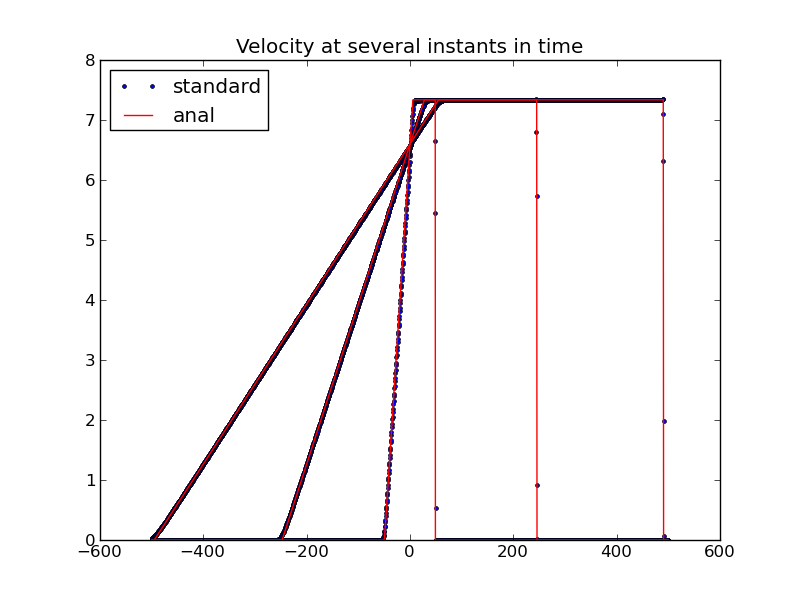
\includegraphics[width=0.9\textwidth]{xvel_plot.png}
\end{center}
\caption{Xvelocity results}
\end{figure}


\endinput
